\section{Experiments and Results}
\label{sec:experiments}



\begin{figure}[t]
    \centering
    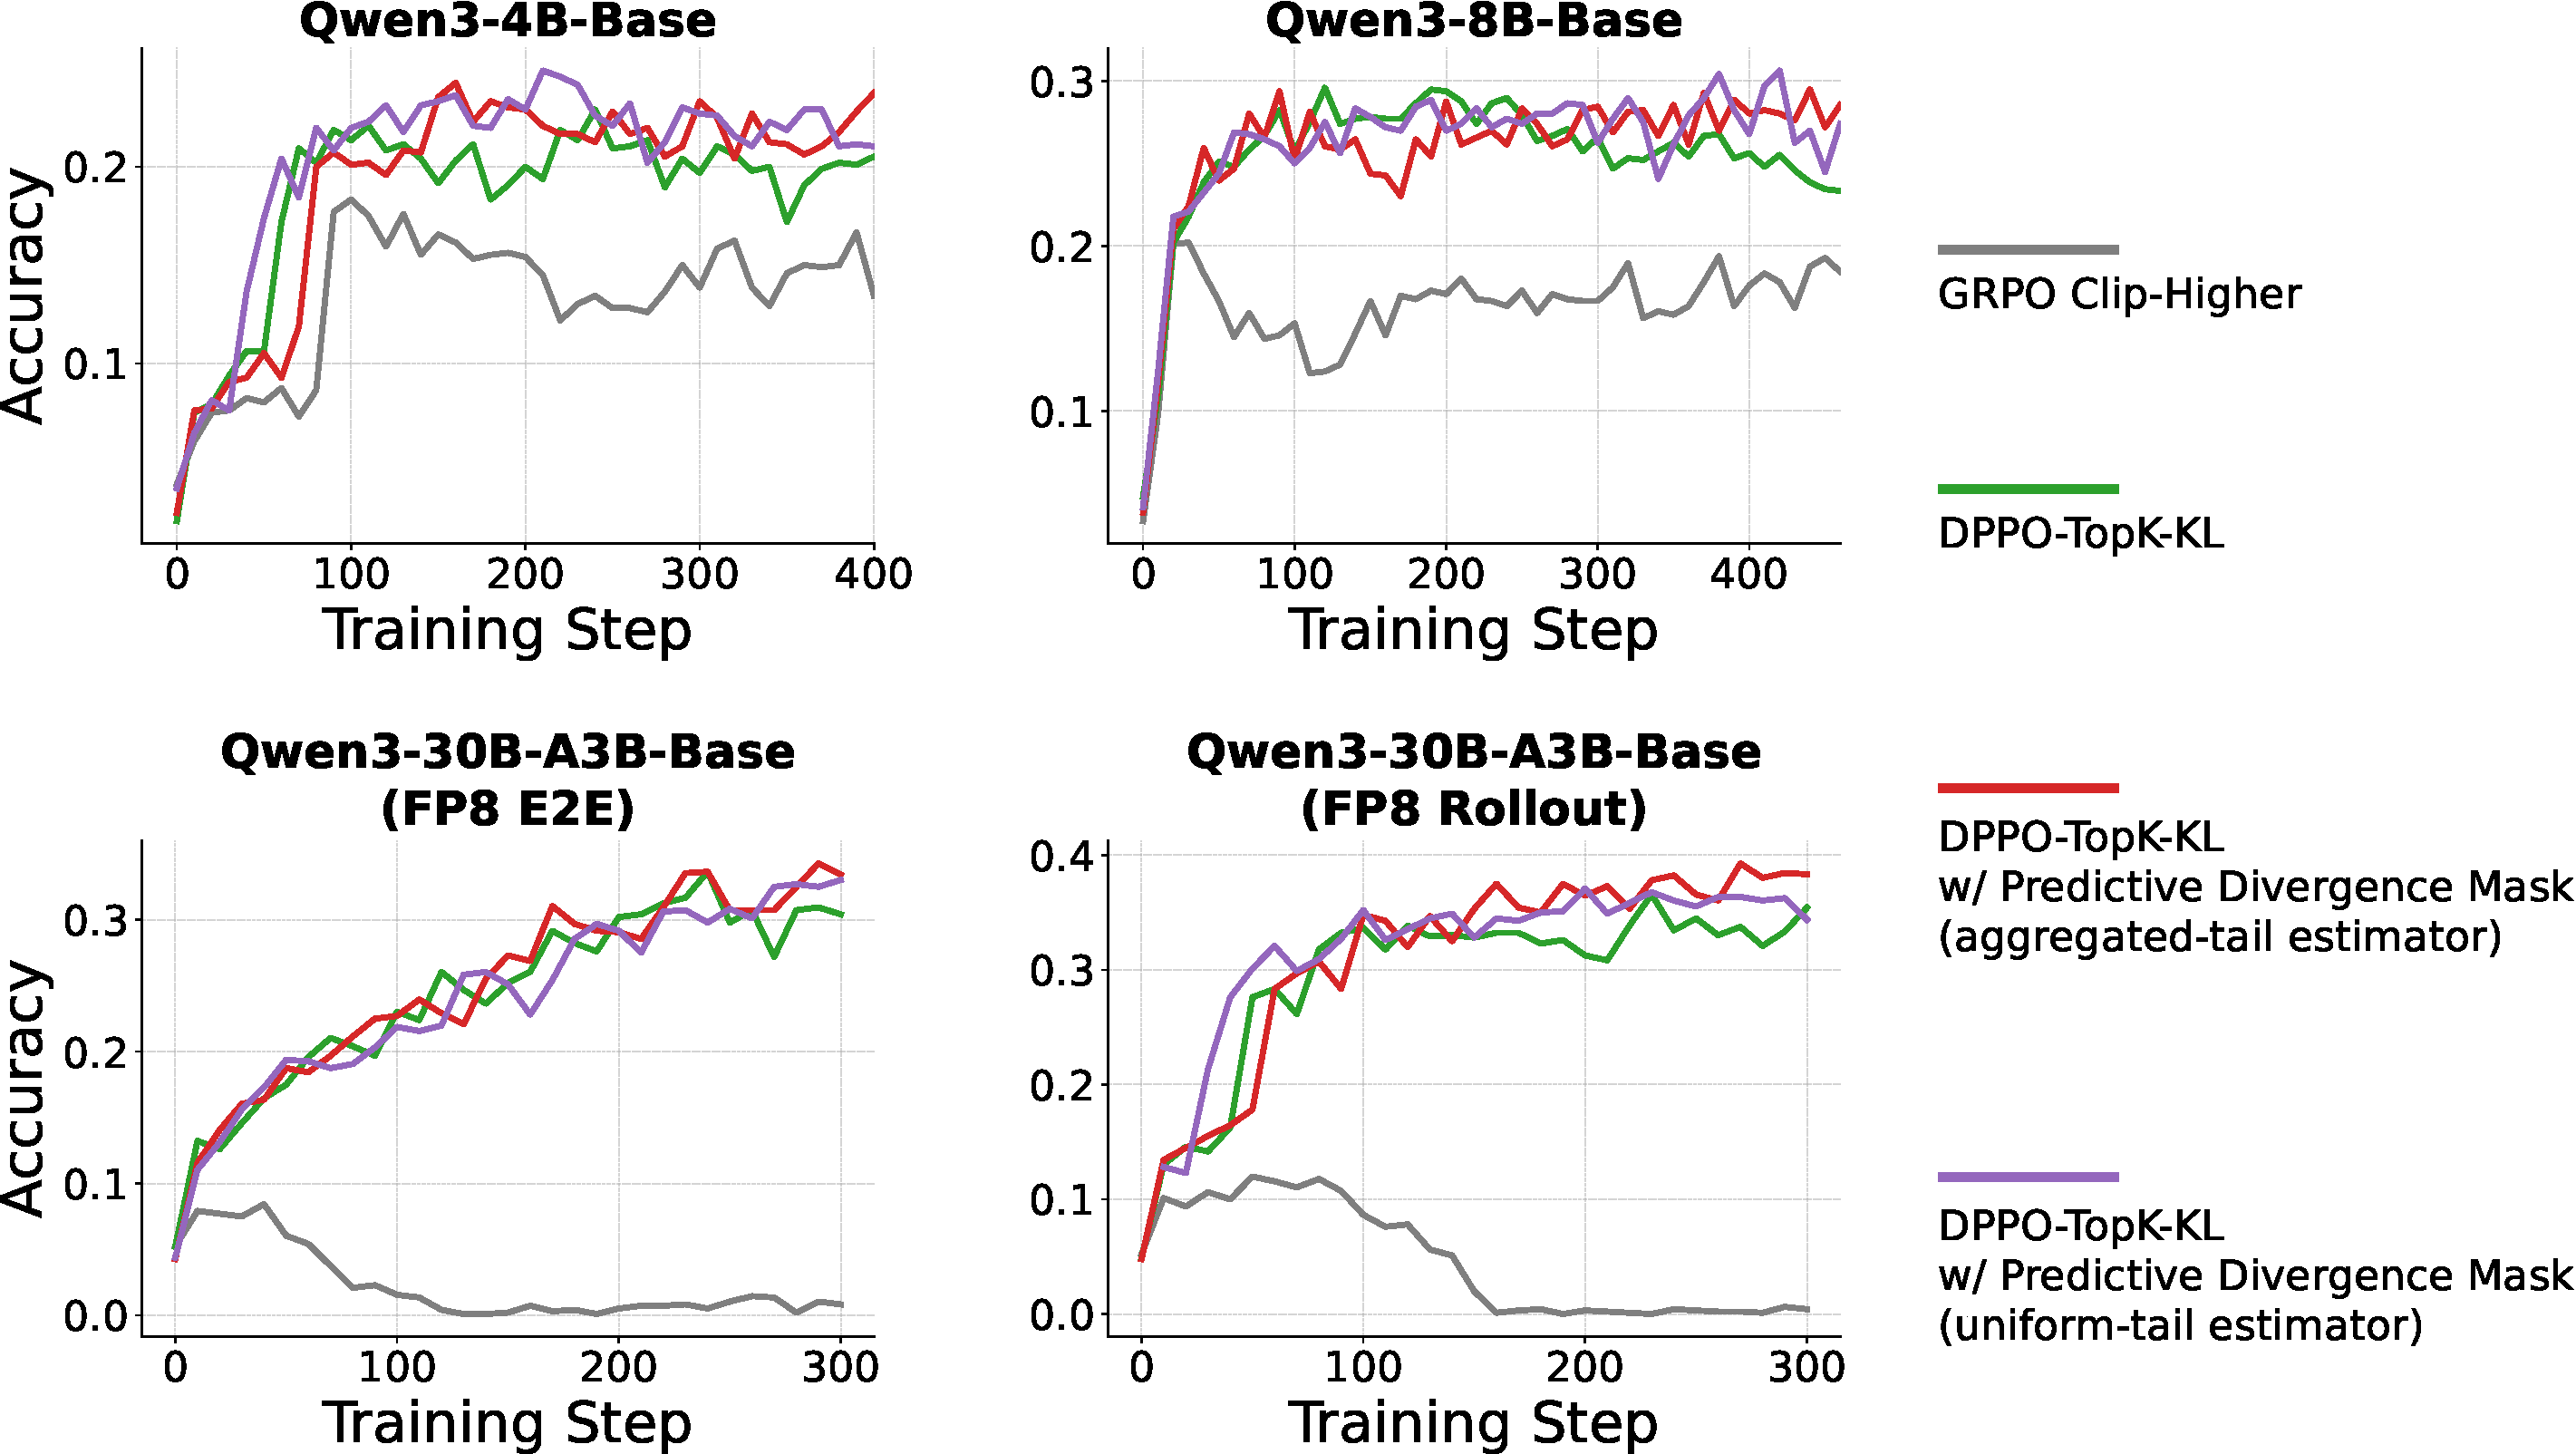
\includegraphics[width=\linewidth]{figs_crop/main_015.pdf}
    \caption{Evaluation accuracy (avg@16, averaged over AIME24 and AIME25) over
    training at $\delta=0.15$ on the four settings: Qwen3-4B-Base, Qwen3-8B-Base, Qwen3-30B-A3B-Base with
    FP8 E2E training, and Qwen3-30B-A3B-Base with FP8 Rollout. The two predictive divergence masks use the aggregated-tail and uniform-tail
estimators for the top-$K$ KL directional-derivative coefficient.}
    \label{fig:main_015}
\end{figure}


\begin{figure}[t]
    \centering
    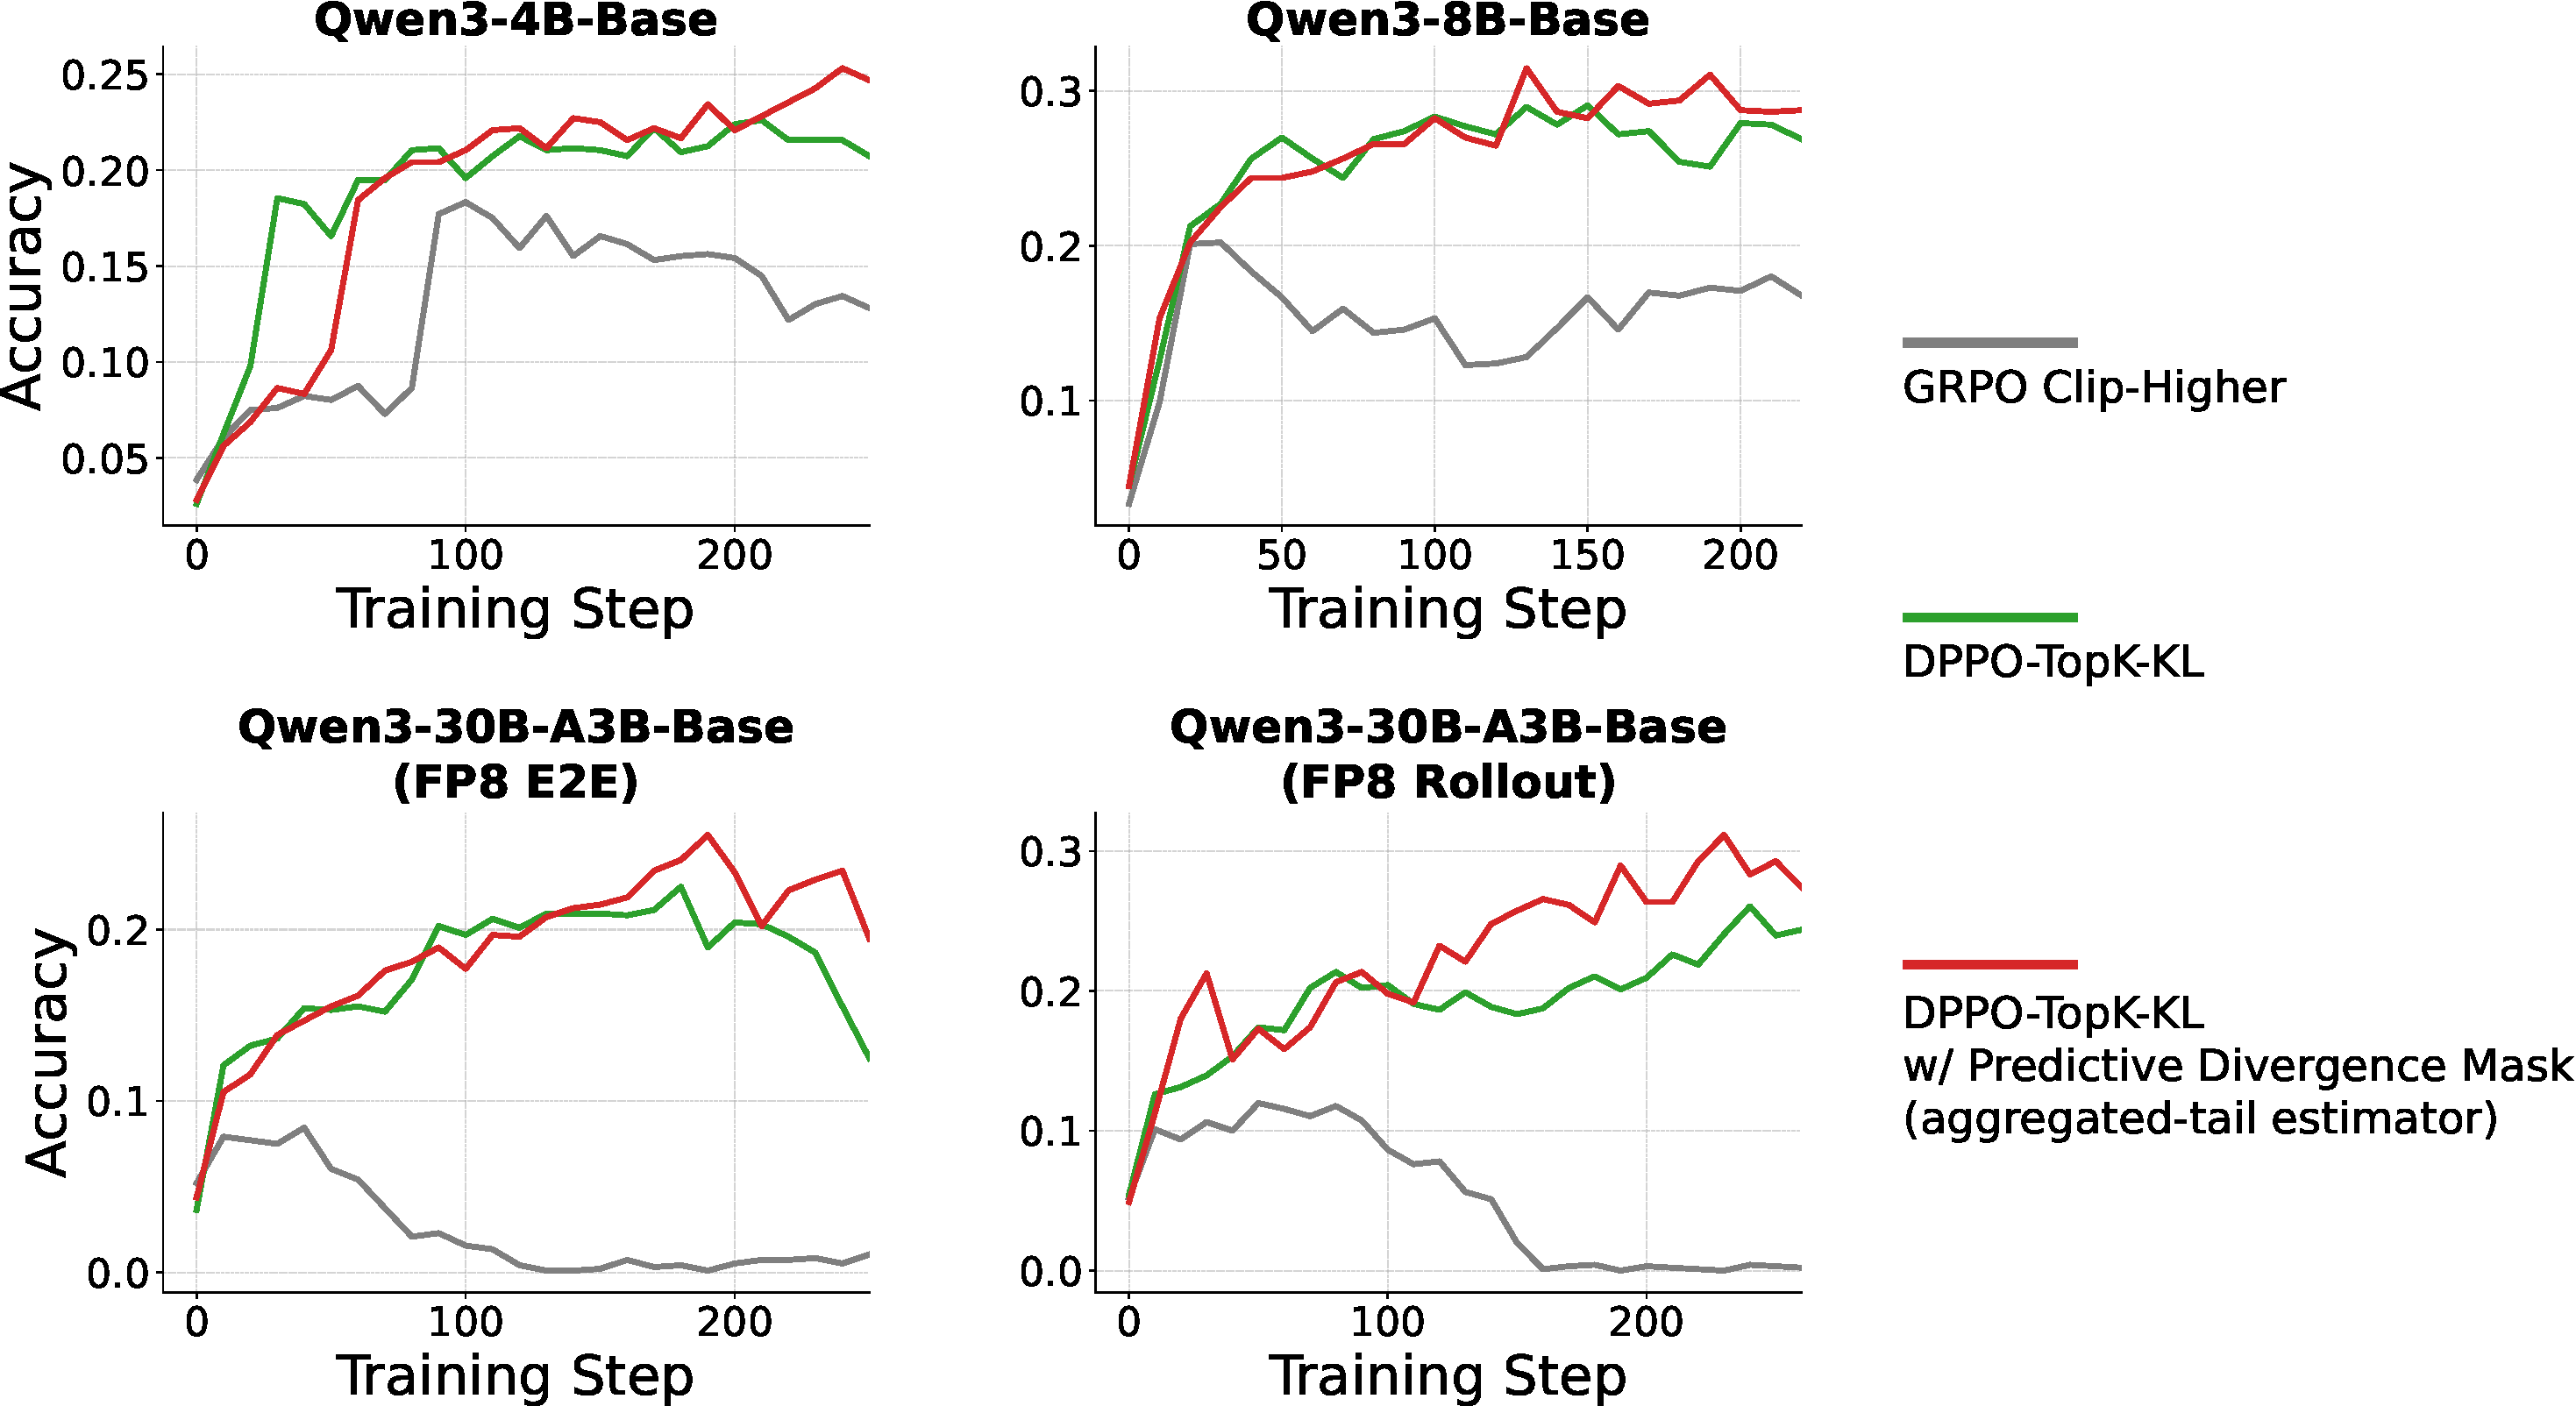
\includegraphics[width=\linewidth]{figs_crop/scaling_weighted_mean16_05.pdf}
    \caption{Evaluation accuracy (avg@16, averaged over AIME24 and AIME25) across the four settings with divergence threshold $\delta=0.05$.}
    \label{fig:main_005}
\end{figure}

\subsection{Main experiment}
\label{sec:exp-setup}

\noindent\textbf{Models, Data, and Benchmarks.} We use a filtered version of DAPO-Math-17k\footnote{\url{https://huggingface.co/datasets/Jiawei415/DPAO_filter}}~\citep{yu2025dapo} as the training dataset, which contains about 13k training samples. In evaluation, we use AIME24 and AIME25 as the benchmarks; for each problem we sample 16 responses and report the average accuracy (avg@16). For the base models, we choose Qwen3-4B-Base, Qwen3-8B-Base, and Qwen3-30B-A3B-Base~\citep{yang2025qwen3} for our experiments. For the Qwen3-30B-A3B-Base model, we use FP8 precision for rollout only (FP8 Rollout) or for both training and rollout (FP8 E2E) to accelerate the training process. FP8 also widens the numerical gap between the rollout and training engines, so these two configurations serve as a stress test. We build on the VeRL framework~\citep{sheng2024hybridflow} for RL training. Experiments are conducted on four nodes, each with 8 NVIDIA H20 GPUs (32 GPUs total).


\noindent\textbf{Methods and Baselines.}
Our primary baseline is DPPO-TopK-KL~\citep{dppo}, which pairs the top-$K$ KL proximity criterion with the original ratio-based direction criterion (Eq.~(\ref{eq:dppo})).
Against it we evaluate two predictive divergence masks, which set the direction from the aggregated-tail estimator (Eq.~(\ref{eq:agg-tail})) and the uniform-tail estimator (Eq.~(\ref{eq:uni-tail})).
We also include GRPO with the clip-higher trick ($\eps_{\mathrm{low}}=0.2$,
$\eps_{\mathrm{high}}=0.28$)~\citep{yu2025dapo} as a ratio-clipping reference. 
All divergence-based methods use $K=20$.
The main comparison uses the recommended $\delta=0.15$, and a threshold-sensitivity study uses $\delta=0.05$. 
Remaining hyperparameters and hardware details are given in Appendix~\ref{app:experiments} and Table~\ref{tab:hyperparameters}.



\noindent\textbf{Main results.}
Figure~\ref{fig:main_015} reports the main comparison at the recommended
threshold $\delta=0.15$.
Across all four model--precision settings, GRPO clip-higher is unstable and
collapses in the two Qwen3-30B-A3B-Base settings, while the divergence-based
methods remain stable.
Within the divergence-based family, the two predictive divergence masks improve over DPPO-TopK-KL.
This comparison isolates the effect of the direction criterion, since DPPO-TopK-KL uses the same top-$K$ KL proximity criterion and differs only in whether the direction is read from the sampled ratio or predicted from the divergence change.
The improvement is therefore consistent with the central hypothesis of the paper:
when the trust region is defined by a divergence, the direction criterion should track the divergence itself rather than the sampled-token ratio.

The aggregated-tail and uniform-tail masks behave very similarly during
training, as expected from the small tail correction of Eq.~(\ref{eq:tail-gap}).
This suggests that the predictive mask is not sensitive to the particular tail
model used to estimate the directional-derivative coefficient.
At the tighter threshold $\delta=0.05$, all methods perform worse, indicating
that this trust region is overly restrictive (Figure~\ref{fig:main_005}).
Even under this tight threshold, however, the predictive divergence masks still
improve over DPPO-TopK-KL, suggesting better robustness to the trust-region
hyperparameter.

\subsection{Analysis of direction criteria}
\label{sec:direction_analysis}

\noindent\textbf{Token-level setup.}
We next examine the direction criterion itself at the token level.
The predictive and ratio-based masks share the same top-$K$ KL proximity
criterion, so they can differ only after a token has already left the trust region.
We therefore restrict the analysis to tokens with
$D=\KLtopk(\bmu\,\|\,\tpi)>\delta$.
For such a token, the ratio-based direction criterion keeps the update when
$\Adv\,(r-1)\le 0$.
The divergence-based direction criterion keeps it when
$\Adv\cdot\Taylor\le 0$, where $\Taylor$ is the estimated first-order
change of the top-$K$ divergence.

To evaluate these decisions, we compare them against the realized divergence
change after one actual update on the same batch,
$\Delta D=D_{\text{post}}-D_{\text{pre}}$.
If $\Delta D>0$, the kept update pushed the token further outside the trust region and should have been masked.
If $\Delta D<0$, the divergence contracted and the kept update was corrective.
We run $61$ independent seeds.
Each seed uses a fresh rollout of $1024$ sequences and applies each mask to the same batch.
Unless otherwise stated, error rates are computed per seed and reported as mean $\pm$ standard error.

\begin{figure}[t]
    \centering
    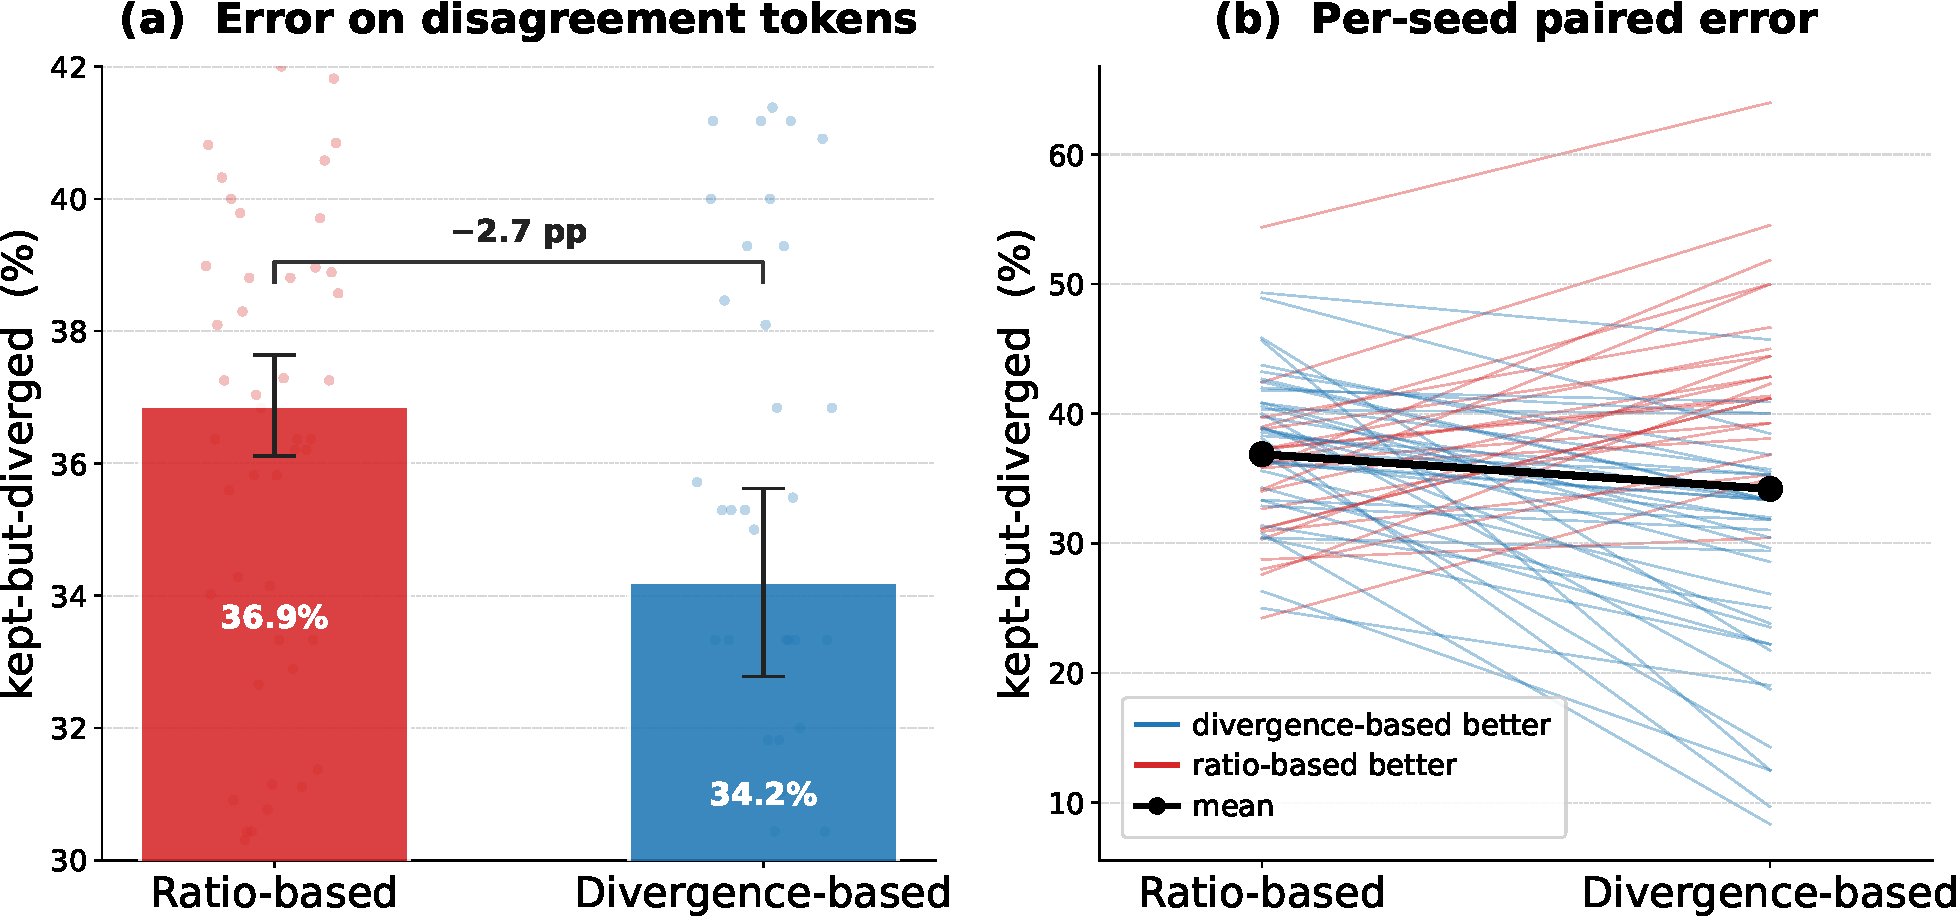
\includegraphics[width=0.9\linewidth]{figs_crop/disagreement_error.pdf}
    \caption{\textbf{Unsafe-keep rate on disagreement tokens}
    ($\delta=0.15$, $61$ seeds). We consider tokens outside the trust region
    ($D>\delta$) on which the ratio-based and divergence-based direction criteria
    make opposite keep/clip decisions. For each criterion, among the disagreement
    tokens it keeps, we report the fraction whose divergence increases after the
    update ($\Delta D>0$). Lower is better. \textbf{(a)} Mean unsafe-keep rate
    across seeds. The divergence-based direction criterion is lower than the
    ratio-based criterion ($34.2\%$ vs.\ $36.9\%$). Error bars show standard
    errors. \textbf{(b)} Per-seed paired comparison, with each line corresponding
    to one seed and colored by which criterion has the lower unsafe-keep rate.}
    \label{fig:disagreement_error}
\end{figure}

\begin{figure}[t]
    \centering
    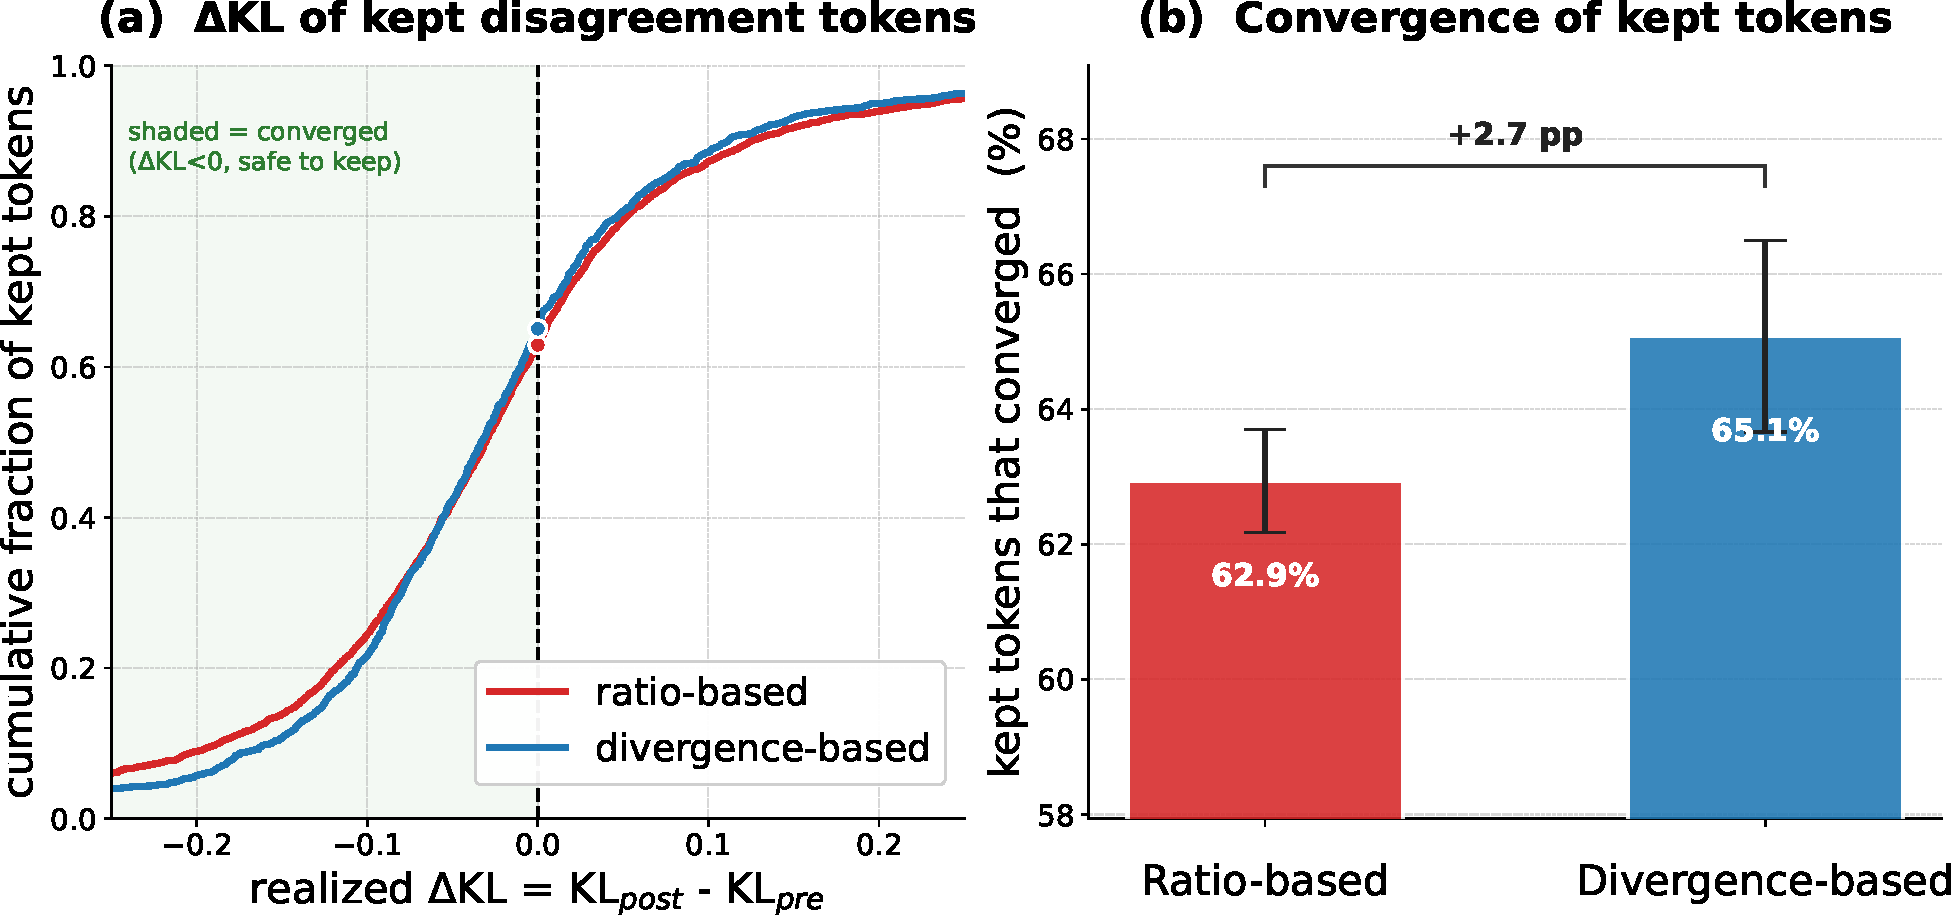
\includegraphics[width=0.9\linewidth]{figs_crop/kept_dkl.pdf}
    \caption{\textbf{Realized divergence change of kept disagreement tokens}
    ($\delta=0.15$, $61$ seeds). For each direction criterion, we collect the
    disagreement tokens it keeps and measure
    $\Delta D=D_{\text{post}}-D_{\text{pre}}$ after one actual update. Tokens from all
    seeds are combined in this figure. \textbf{(a)} Empirical CDF of $\Delta D$.
    The shaded region $\Delta D<0$ indicates kept updates that contracted the
    divergence. \textbf{(b)} Fraction of kept updates with $\Delta D<0$. The
    divergence-based direction criterion keeps a larger fraction of contracting
    updates than the ratio-based criterion ($65.1\%$ vs.\ $62.9\%$).}
    \label{fig:kept_dkl}
\end{figure}

\noindent\textbf{Results.}
On average, each seed contains $1435$ tokens outside the trust region.
The two direction criteria agree on the keep/clip decision for most of them and
disagree on only about $82$ tokens per seed.
Thus the two masks are distinguishable only on a small disagreement set, which is
where Figures~\ref{fig:disagreement_error}--\ref{fig:kept_dkl} focus.

Figure~\ref{fig:disagreement_error} measures unsafe keeps.
Among disagreement tokens kept by each criterion, the unsafe-keep rate is the
fraction whose divergence later increases.
Averaged over seeds, this rate is lower for the divergence-based direction
criterion than for the ratio-based direction criterion ($34.2\%$ vs.\ $36.9\%$),
a $2.7$ percentage-point reduction.
The divergence-based criterion has the lower unsafe-keep rate on $38$ of the
$61$ seeds.

Figure~\ref{fig:kept_dkl} shows the same comparison from the corrective side.
After combining tokens from all seeds, the fraction of kept updates that contract
the divergence is higher for the divergence-based direction criterion
($65.1\%$ vs.\ $62.9\%$).
This statistic is not the exact complement of the per-seed unsafe-keep rate in
Figure~\ref{fig:disagreement_error}, because it combines tokens across seeds before
computing the fraction.
The two figures therefore provide complementary views of the same directional
effect rather than two independent tests.

Overall, the token-level evidence supports the mechanism behind the predictive
mask.
The divergence-based direction criterion is better aligned with the realized
change of the divergence than the sampled-token ratio, although the effect is
modest because the disagreement set is small.
